\subsection{Threat Model}\label{threat-model}
The type of attack that time randomization seeks to thwart has the following properties:
\begin{itemize}\addtolength{\itemsep}{-.35\baselineskip}
	\item The attack targets a concurrency bug.
	\item The attacker can gain knowledge about the relative timing between two
  or more threads relevant to the bug.
	\item The attacker leverages this knowledge to craft the attack.
\end{itemize}
Note that there are many ways to gain knowledge about relative thread timing, including results from fuzzing experiments.
In the case that the fuzzing is done on a binary, it may not even be obvious how many threads are involved.
Nevertheless, positive fuzzing results can be considered knowledge about relative thread timing which can then be used to craft an attack.

As an example, consider the following scenario:
A remote attacker is communicating with some server software, and has somehow become aware of a concurrency bug in that software.
They have devised a way to exploit the bug, which includes a method for inducing a buggy thread interleaving.
For concreteness, let's assume that the bug is exposed when a save operation
is attempted by one thread during the critical section of another save
operation in another thread (e.g., after some checking has been done, but before the results have been used, sometimes referred to as a time of check to time of use attack).
If the server immediately spawns threads to execute save operations in response to client requests, the attacker's work consists of identifying the proper delay between two save threads such that the critical sections intersect.
The critical sections in this context are sometimes referred to as a vulnerability window~\cite{Yang2012}.

If the server software is available to the attacker, they can simply study it on a similar system (which they control) to determine the appropriate delay required to expose the bug.
Armed with this knowledge, they stand a good chance of exploiting the bug on the target system by sending requests with the same delay.
\begin{figure*}
	\centering
	\begin{subfigure}{\columnwidth}
		\fbox{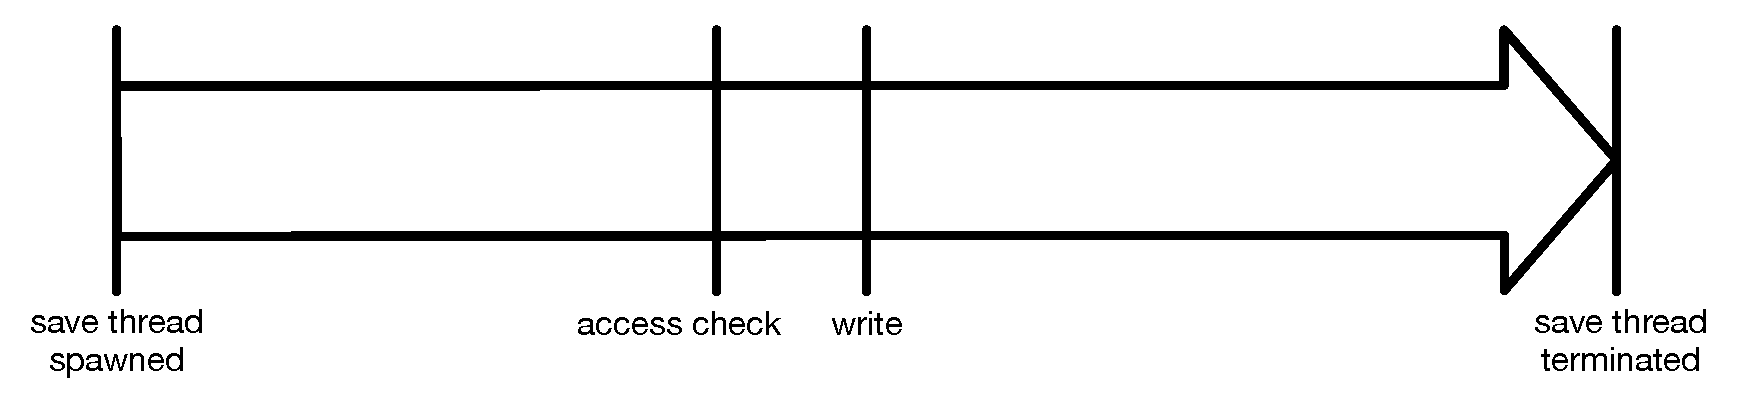
\includegraphics[width=.95\textwidth]{figures/save_op}}
		\caption{}
		\label{fig_save_op}
	\end{subfigure}
	\begin{subfigure}{\columnwidth}
		\fbox{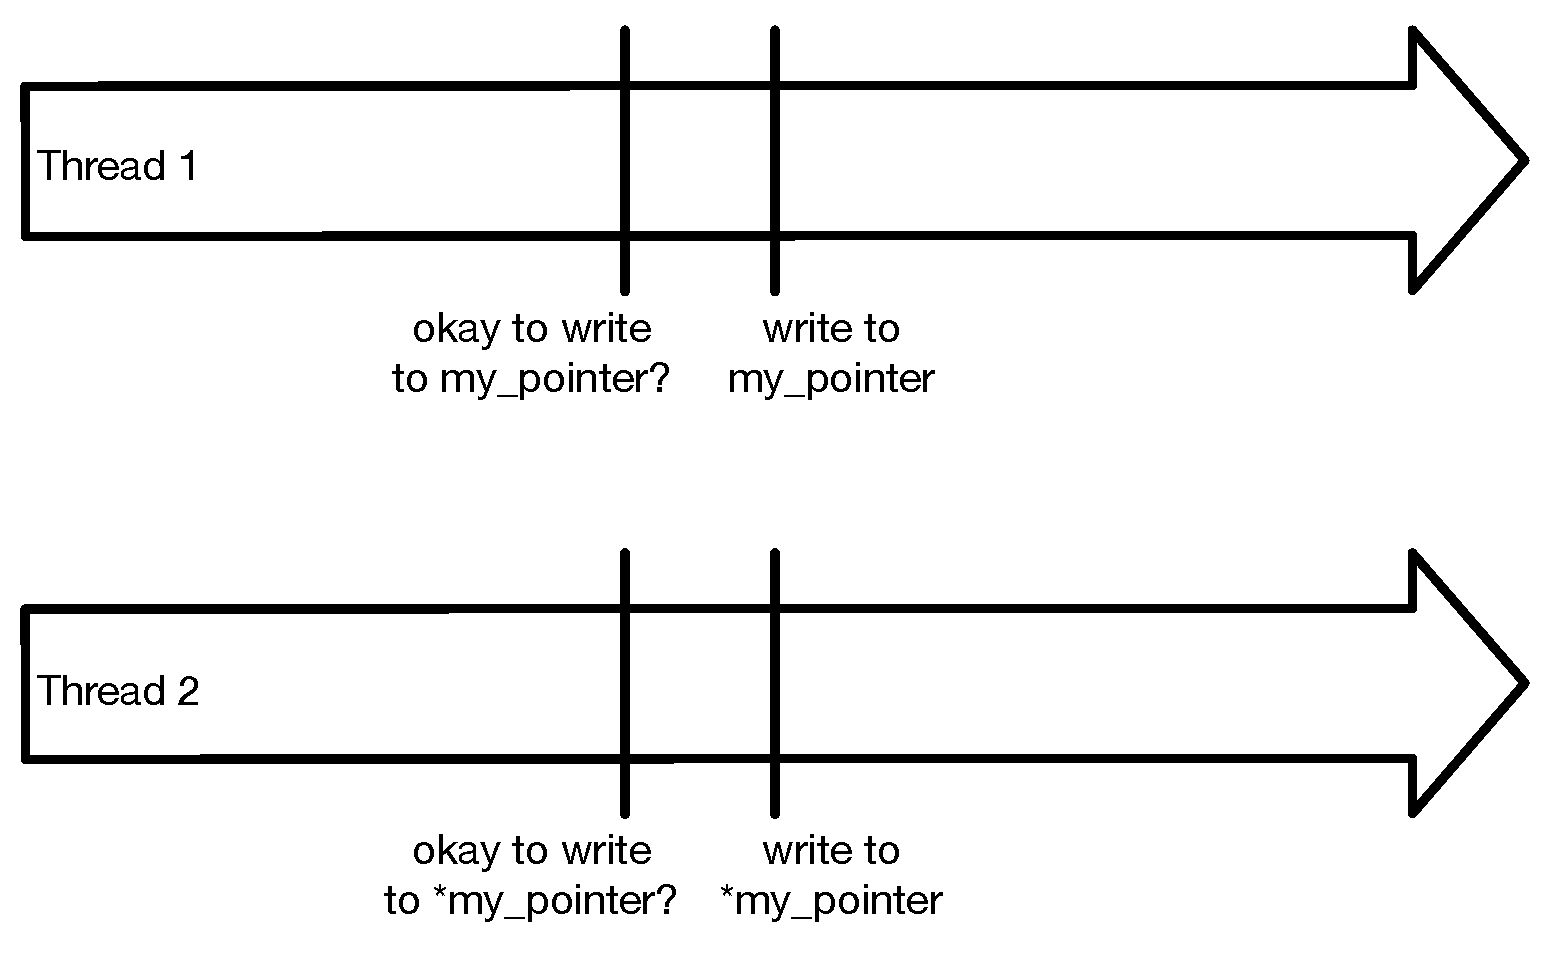
\includegraphics[width=.95\textwidth]{figures/two_threads}}
		\caption{}
		\label{fig_two_threads}
	\end{subfigure}
	\begin{subfigure}{\columnwidth}
		\fbox{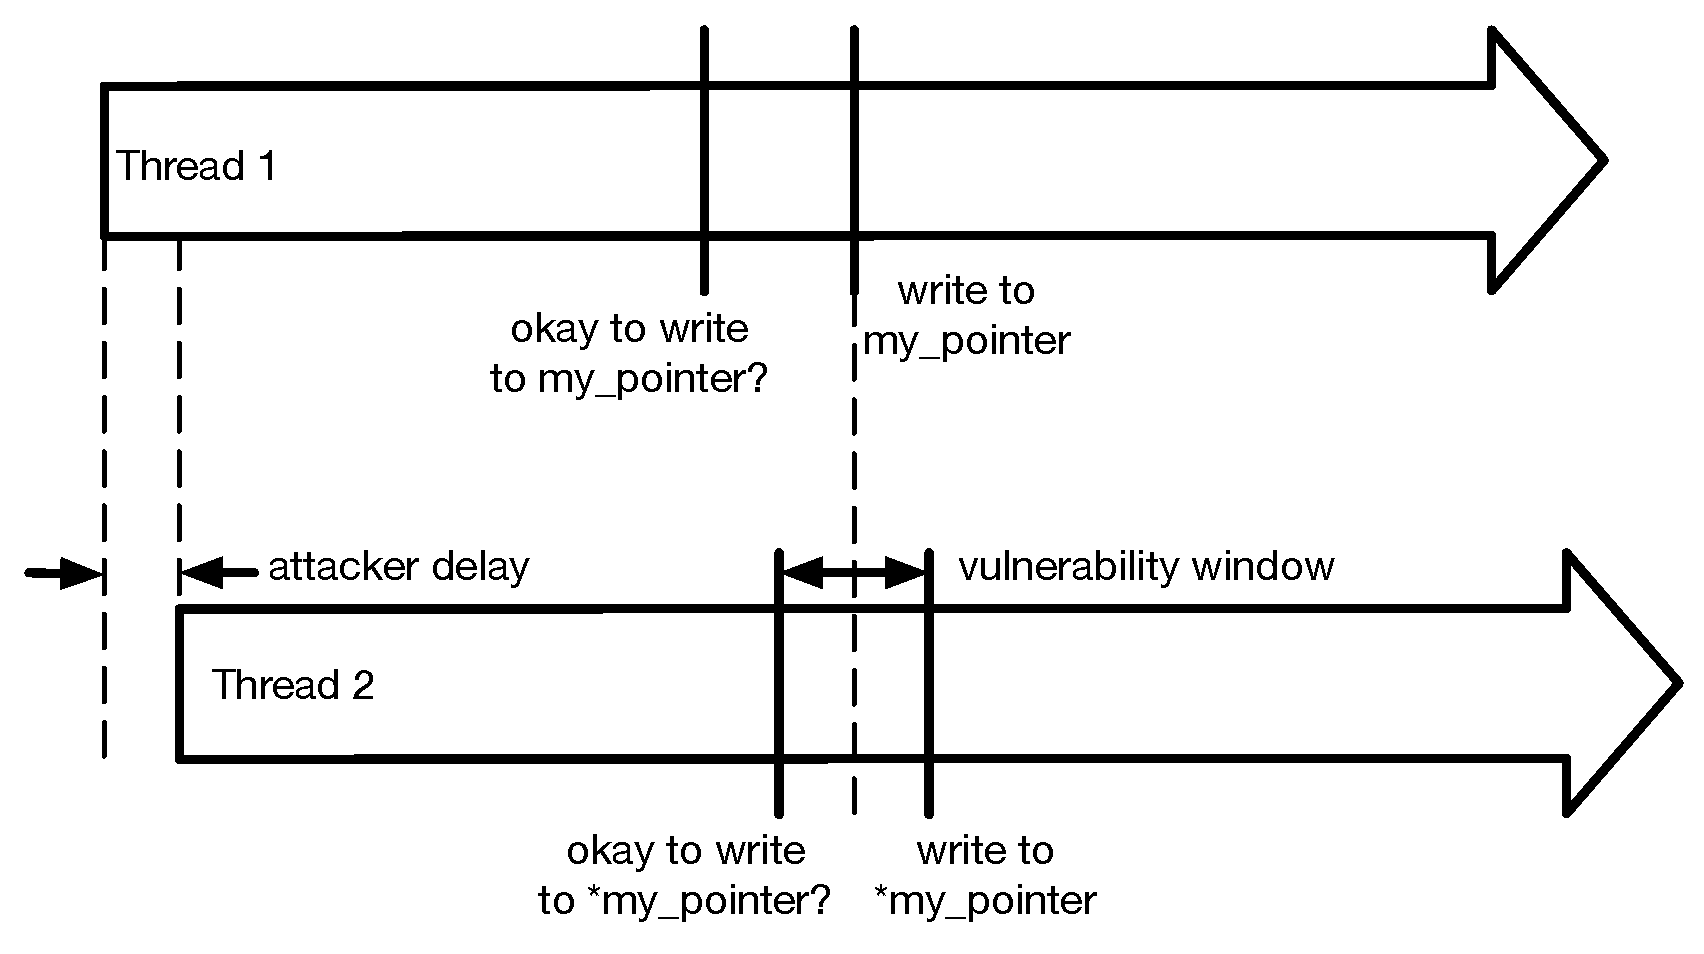
\includegraphics[width=.95\textwidth]{figures/attack}}
		\caption{}
		\label{fig_attack}
	\end{subfigure}
	\begin{subfigure}{\columnwidth}
		\fbox{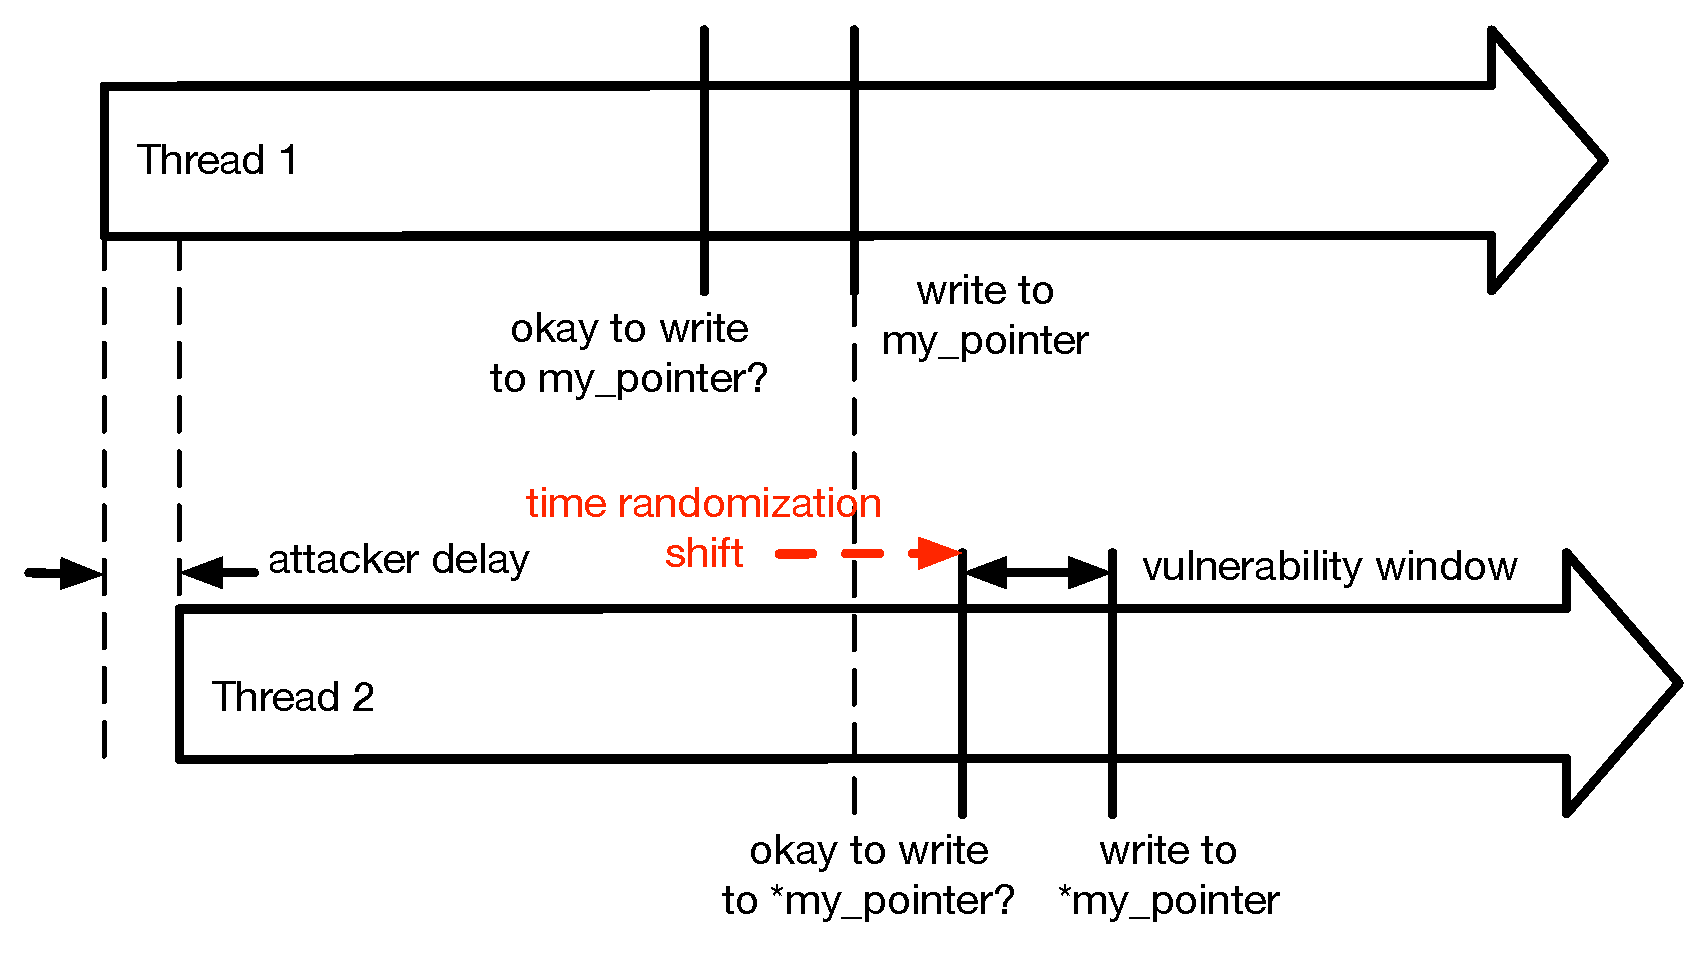
\includegraphics[width=.95\textwidth]{figures/thwart}}
		\caption{}
		\label{fig_thwart}
	\end{subfigure}
	\caption{
		A pictorial representation of the example concurrency attack described in \autoref{threat-model}.
		(\ref{fig_save_op}): A single save operation thread with two significant points---an access check where the thread checks whether the requestor has the proper access rights to make the requested change, and a write where the requested change is made (assuming the access check succeeds).
		(\ref{fig_two_threads}): Two save operation threads.
		Thread 1 is saving to the (poorly designed) global variable \texttt{my\_pointer}.
		Thread 2 is saving to the memory location indicated by \texttt{my\_pointer}.
		We can see the makings for a TOCTOU attack here---if \texttt{my\_pointer} points to a memory location to which the attacker has access, the check in Thread 2 will succeed; but if Thread 1 modifies \texttt{my\_pointer} to point to another memory location to which the attacker should not have access before Thread 2 writes, Thread 2 will write to that memory location.
		An attacker has thus achieved privilege escalation.
		(\ref{fig_attack}): In fact, if the thread timing (i.e., the timing between thread spawn and the significant points labeled in (\ref{fig_save_op}), and the relative timing between Thread 1 and Thread 2) are predictable, the attacker can study that thread timing on another system that they control.
		They can then determine an appropriate delay between spawning Thread 1 and Thread 2 such that the write to \texttt{my\_pointer} by Thread 1 falls inside the vulnerability window of Thread 2.
		(\ref{fig_thwart}): An example result of time randomization.
		Here, time randomization has shifted the vulnerability window of Thread 2 with respect to the write by Thread 1 such that the delay calculated by the attacker in (\ref{fig_attack}) no longer aligns the two.
		This result can be achieved, for example, by a time randomization transformation which adds a delay between the spawning of Thread 2 and the access check by Thread 2.
		Note that a delay between the spawning of Thread 1 and the write by Thread 1 would also cause the write to miss the vulnerability window in Thread 2.
	}
	\label{fig_exploitation}
\end{figure*}
\subsection{Implementation}\label{implementation}
Time randomization, the randomization of synchronization schedules and thread interleavings, as well as the relative timing between and among threads, aims to make this type of attack much harder.
By making the relative timing between threads less predictable, the cost of carrying out the attack above is dramatically increased.
Figure~\ref{fig_exploitation} presents a graphical explanation of this attack and one possible result of time randomization that would cause it to fail.

Of the various software diversity transformations which have been studied~\cite{Larsen2014}, the ones which are most applicable to time randomization are those which
\begin{itemize}\addtolength{\itemsep}{-.35\baselineskip}
	\item add delays to a thread or threads, and those which
	\item reorder something such that thread interleaving is affected.
\end{itemize}
The first category is almost always possible, as adding delays rarely breaks programs.
However, an obvious drawback to this approach is loss of performance, and this drawback must be weighed against the benefits of the transformation.
In the second case, the ``something'' reordered can be at any granularity (instruction level, function level, program level, etc.) so long as thread interleaving is affected.
These types of transformations are less likely to have performance costs, but they are more likely to break the correctness of programs.
This work studies three transformations in the first category.

The three transformations for introducing automated diversity explored in the context of concurrency attacks in this work consist of interposing external library calls~\cite{Conrad2009} made by the software to be protected each with random numbers of inline assembly NOP instructions.
This was accomplished by first specifying a max delay (per interposition).
Then, for each of the external library functions chosen for interposition, a random integer between zero and the max delay was selected.
Finally, that number was used as the loop limit on a loop of assembly NOPs for that external library function.
The interpositions of the NOP loops were compiled into a dynamic library file, and that file was specified to be preloaded with the LD\_PRELOAD environment variable.

The three transformations vary only in the way that the library functions are chosen for interposition.
The first transformation chooses all external library function calls indiscriminately, while the other two use synchronization mechanisms to indicate locations where delays may have the greatest effect on relative thread timing.
In all transformations, \texttt{ltrace}~\cite{cespedesltrace} is run on the unmodified program to be protected while it is being subjected to an exploit attempt.
Using the log from that ltrace run,
\begin{description}\addtolength{\itemsep}{-.35\baselineskip}
	\item[T1] the first transformation chooses every external library function call for interposition,
	\item[T2] the second transformation chooses every external library function call immediately preceding a synchronization mechanism, and
	\item[T3] the third transformation chooses every external library function call immediately following a synchronization mechanism.
\end{description}
(Hereafter, these transformations are referred to as \textbf{T1}, \textbf{T2}, and \textbf{T3}.)
Functions were only excluded in the rare cases that the function takes a
variable argument list, or interposing the function interferes with the
interposition method itself (e.g., \texttt{sigsetjmp}).
Both cases are unsuitable for the interposition method used in this work.
As all of the experiments were conducted on Linux, ``synchronization
mechanisms'' were generally identified as \texttt{pthread} function calls, except for the case of Libvirt which redefines its own synchronization mechanisms.

In addition to the question of the proper diversity transformation, there is also the question of when (or how often) to diversify.
We do not address the latter here, except insofar as the transformations tested here dictate that the diversification must be done prior to load time (so that the interposition library is available for preloading).
As the randomization processes \textbf{T1}-\textbf{T3} require considerable computation, diversification at \textit{each} load time is likely infeasible.
However, one could certainly imagine these transformations being applied at install time, and even possibly at each reboot.